%% COULEURS %%
\section{Gestion des Couleurs}
%gestion des couleurs, color blending, ...
	\begin{frame}{Gestion des Couleurs}
		Reprenons encore une fois notre astronaute à la conférence Solvay:

		\begin{figure}
			\centering
			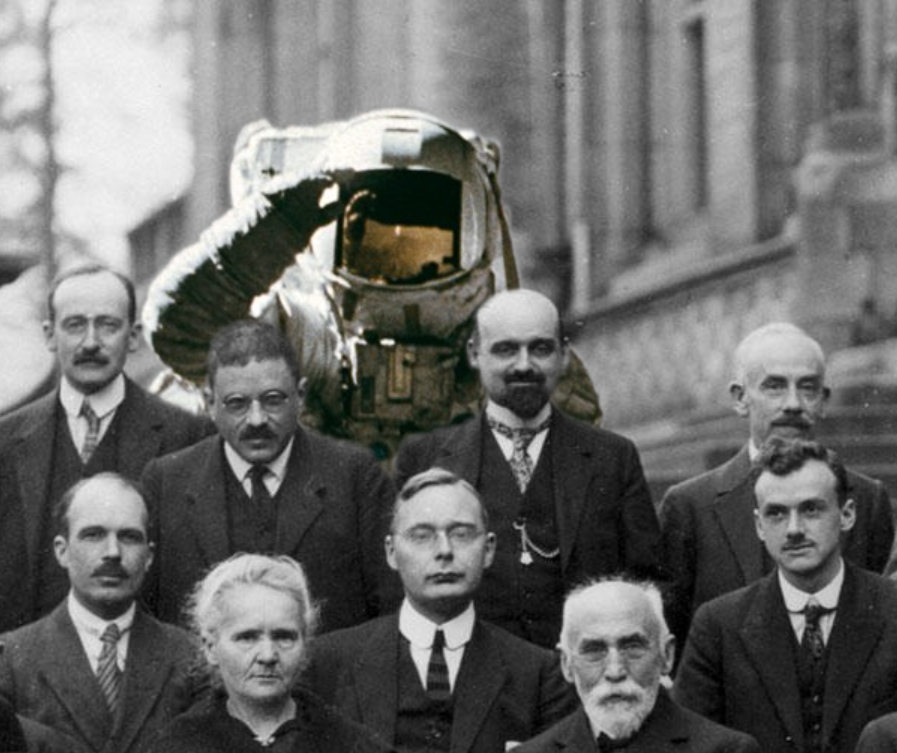
\includegraphics[height=150px]{Images/colours/col1}
		\end{figure}
	\end{frame}

	\begin{frame}{Gestion des Couleurs}
		Noir \& blanc (simple) $\rightarrow$ Désaturer et gérer la luminosité et le contraste (basique).

		Modifications des couleurs $\rightarrow$ \emph{Destructif} $\rightarrow$ Duplication des calques de travail

		\begin{figure}
			\centering
			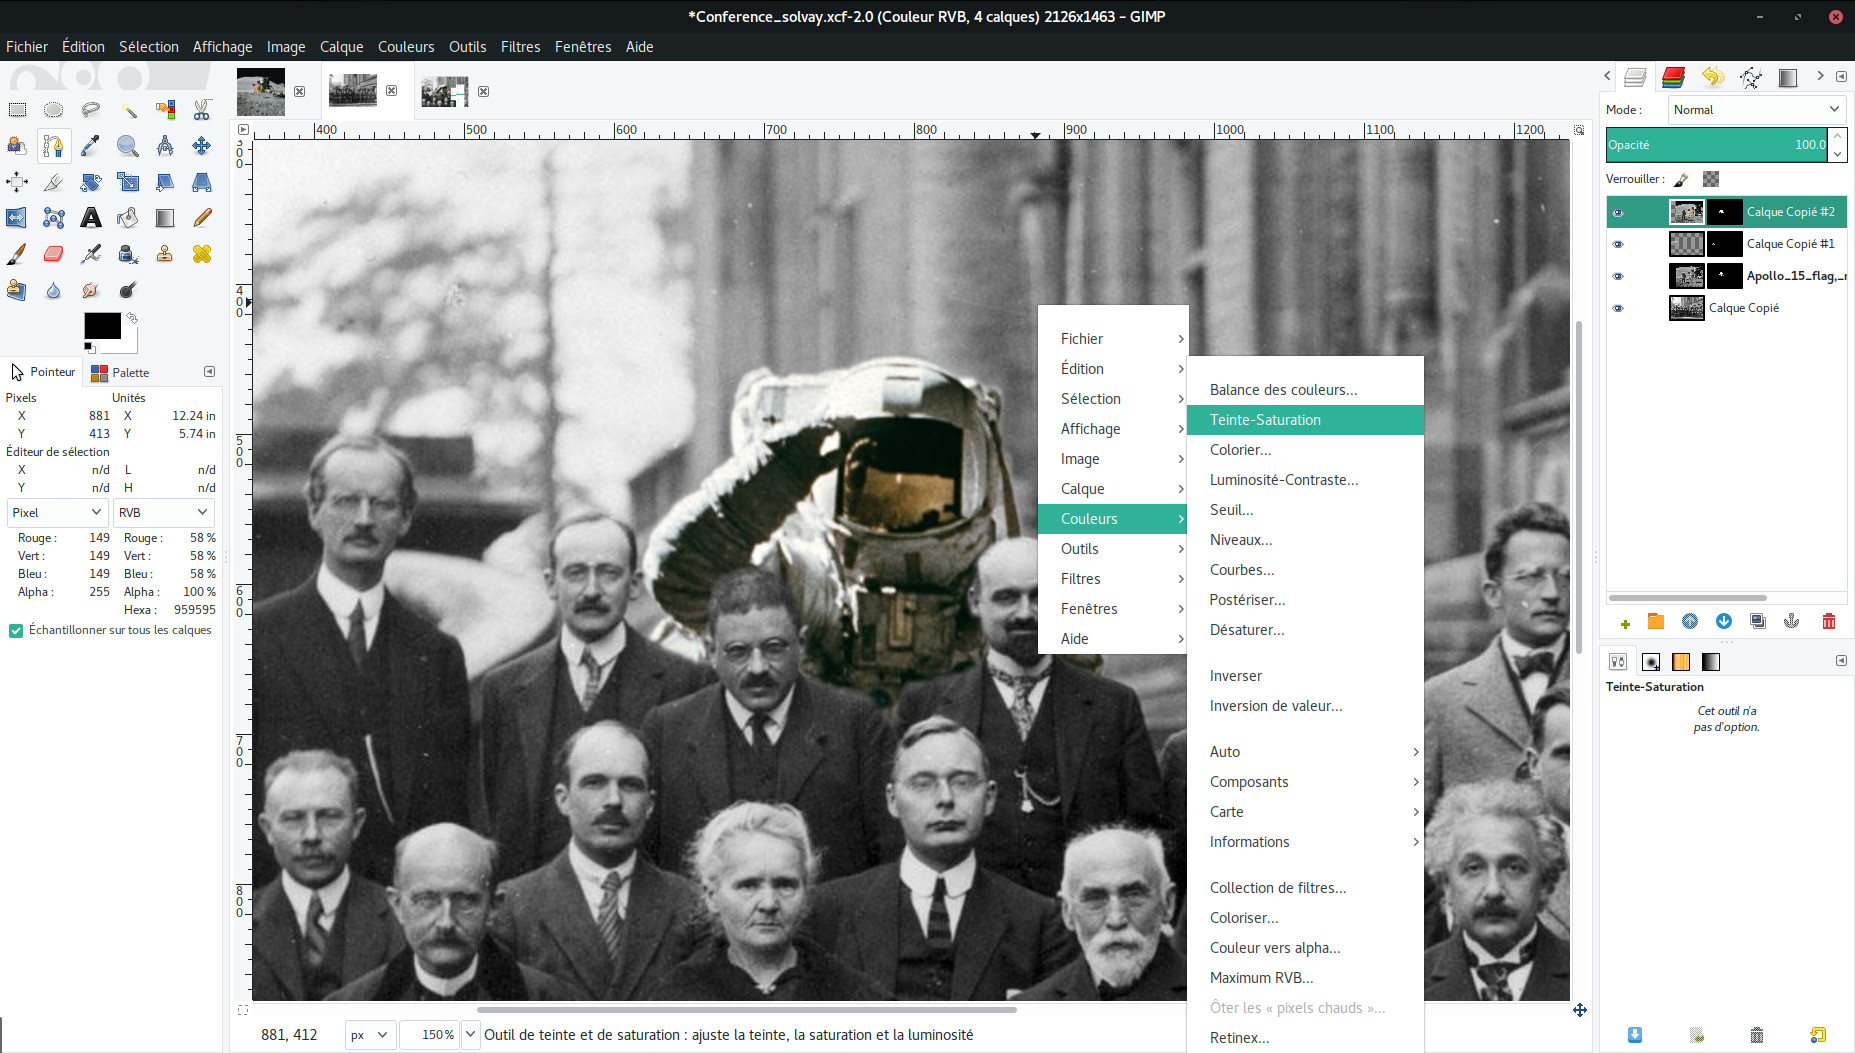
\includegraphics[height=140px]{Images/colours/col2}
		\end{figure}
	\end{frame}

	\begin{frame}{Gestion des Couleurs}

		\begin{figure}[H]
			\centering
			\begin{minipage}{.5\textwidth}
				\centering
				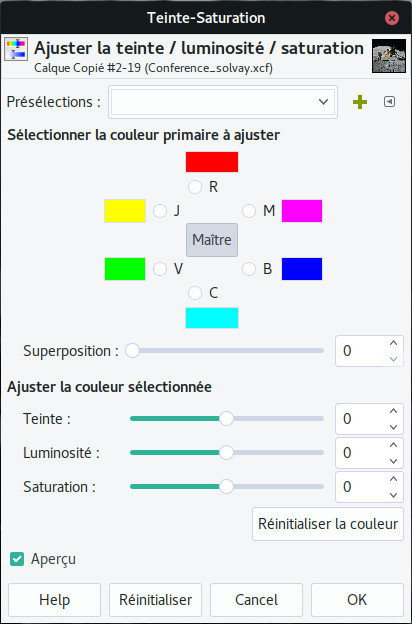
\includegraphics[height=150px]{Images/colours/col3}
				\end{minipage}$\rightarrow$%
			\begin{minipage}{.5\textwidth}
				\centering
				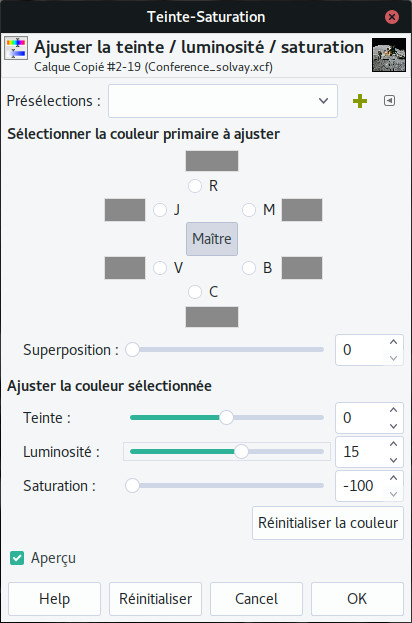
\includegraphics[height=150px]{Images/colours/col4}
				\end{minipage}
			\end{figure}
	\end{frame}

	\begin{frame}{Gestion des Couleurs}
	\textbf{Et comment je peux faire pour changer la couleur d'un élément?}
	Deux techniques:
	\begin{enumerate}
		\item Technique du calque coloré (facile et rapide à mettre en place)
		\item Technique des variations du la balance des blancs (plus précise mais aussi plus fastidieuse)
	\end{enumerate}
		\begin{figure}[H]
			\centering
			\begin{minipage}{.5\textwidth}
				\centering
				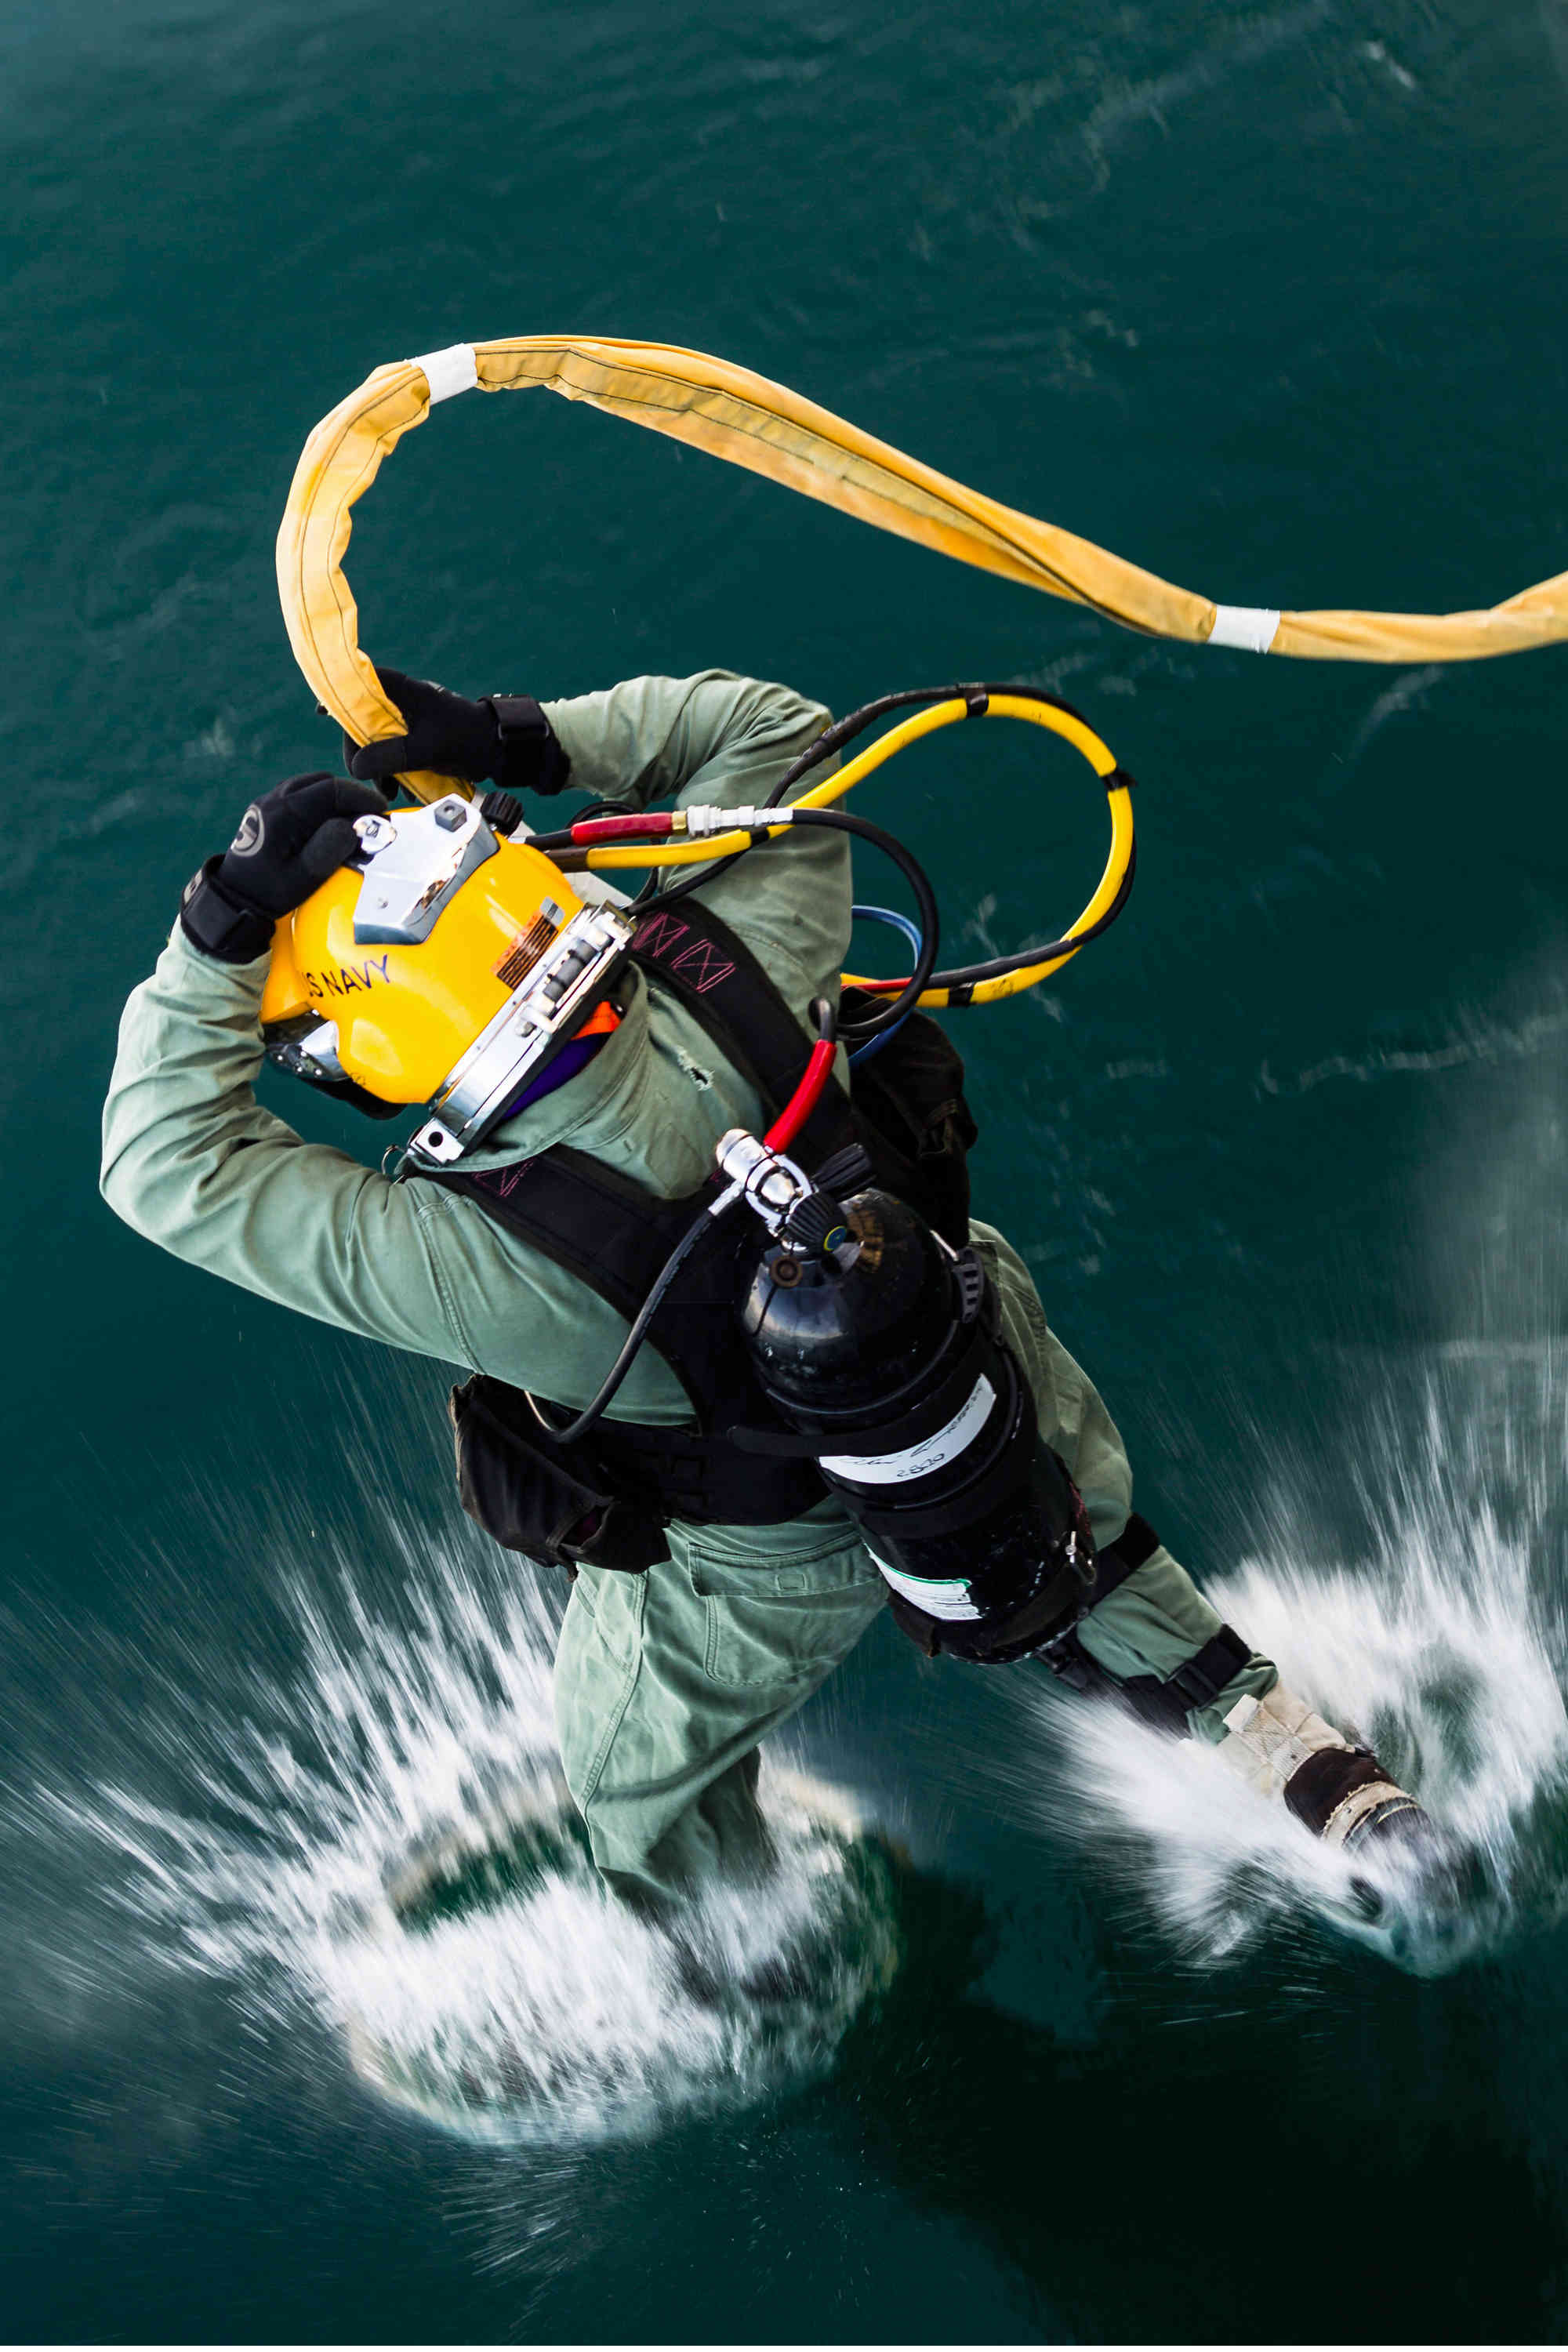
\includegraphics[height=150px]{Images/colours/col5}
				\end{minipage}$\rightarrow$%
			\begin{minipage}{.5\textwidth}
				\centering
				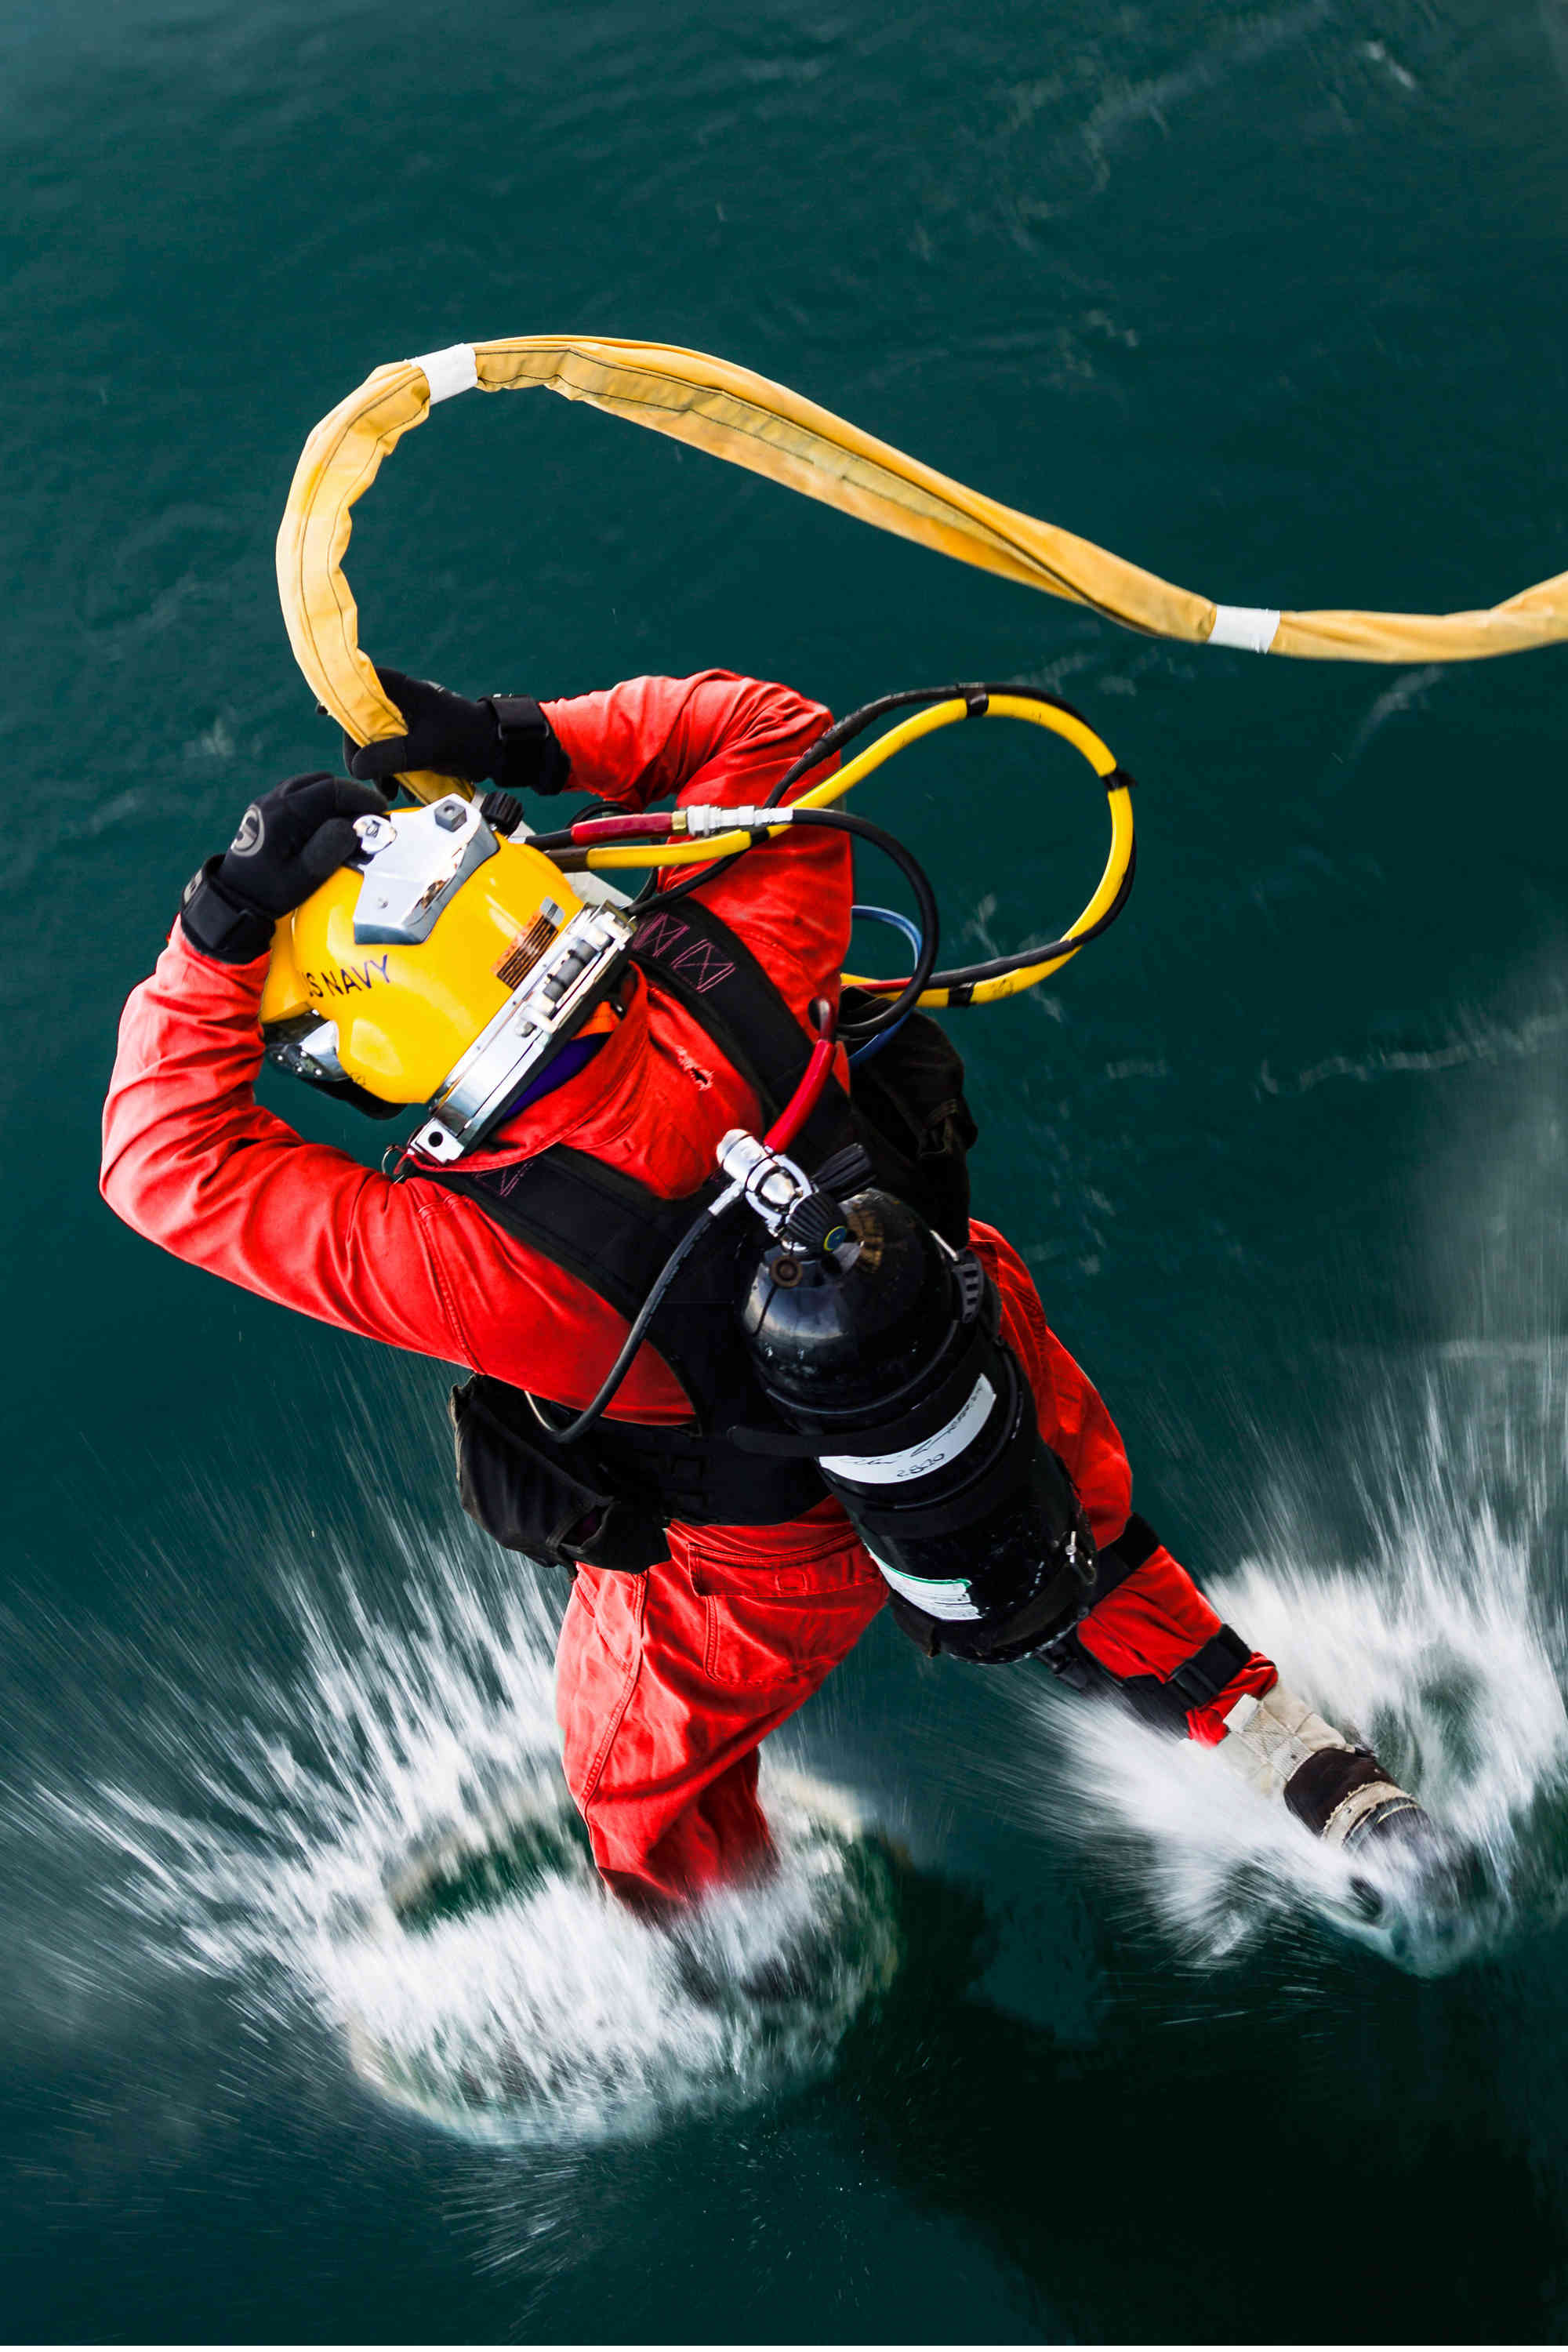
\includegraphics[height=150px]{Images/colours/col6}
				\end{minipage}
			\end{figure}
	\end{frame}

	\begin{frame}{Gestion des Couleurs}
	\framesubtitle{Technique du calque coloré}
		\begin{enumerate}
			\only<1>{
			\item[1.] \textbf{Remplir un calque avec la couleur que l'on souhaite et le masquer pour rendre visible les zones où l'on souhaite changer la couleur}
			\begin{figure}
				\centering
				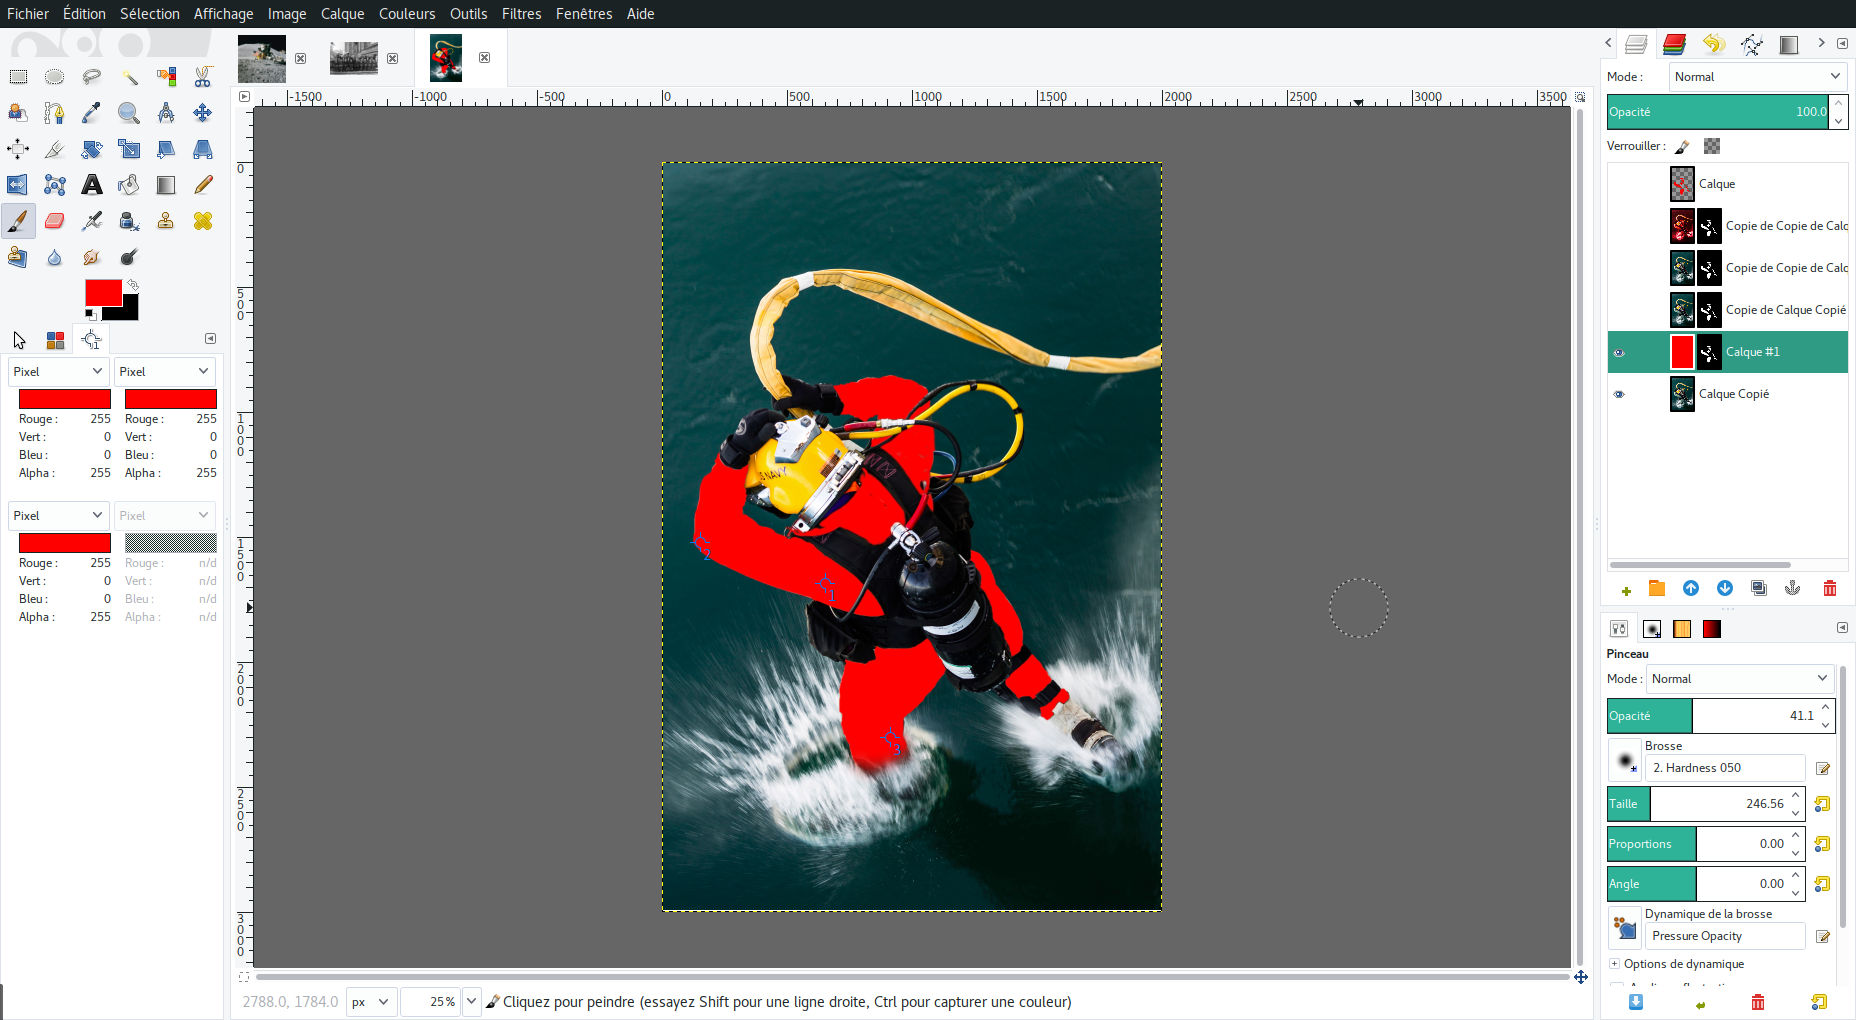
\includegraphics[height=150px]{Images/colours/col7}
			\end{figure}
			}
			\only<2>{
			\item[2.]\textbf{Changer le mode de fusion du masque à "Couleur".}
			\begin{figure}
				\centering
				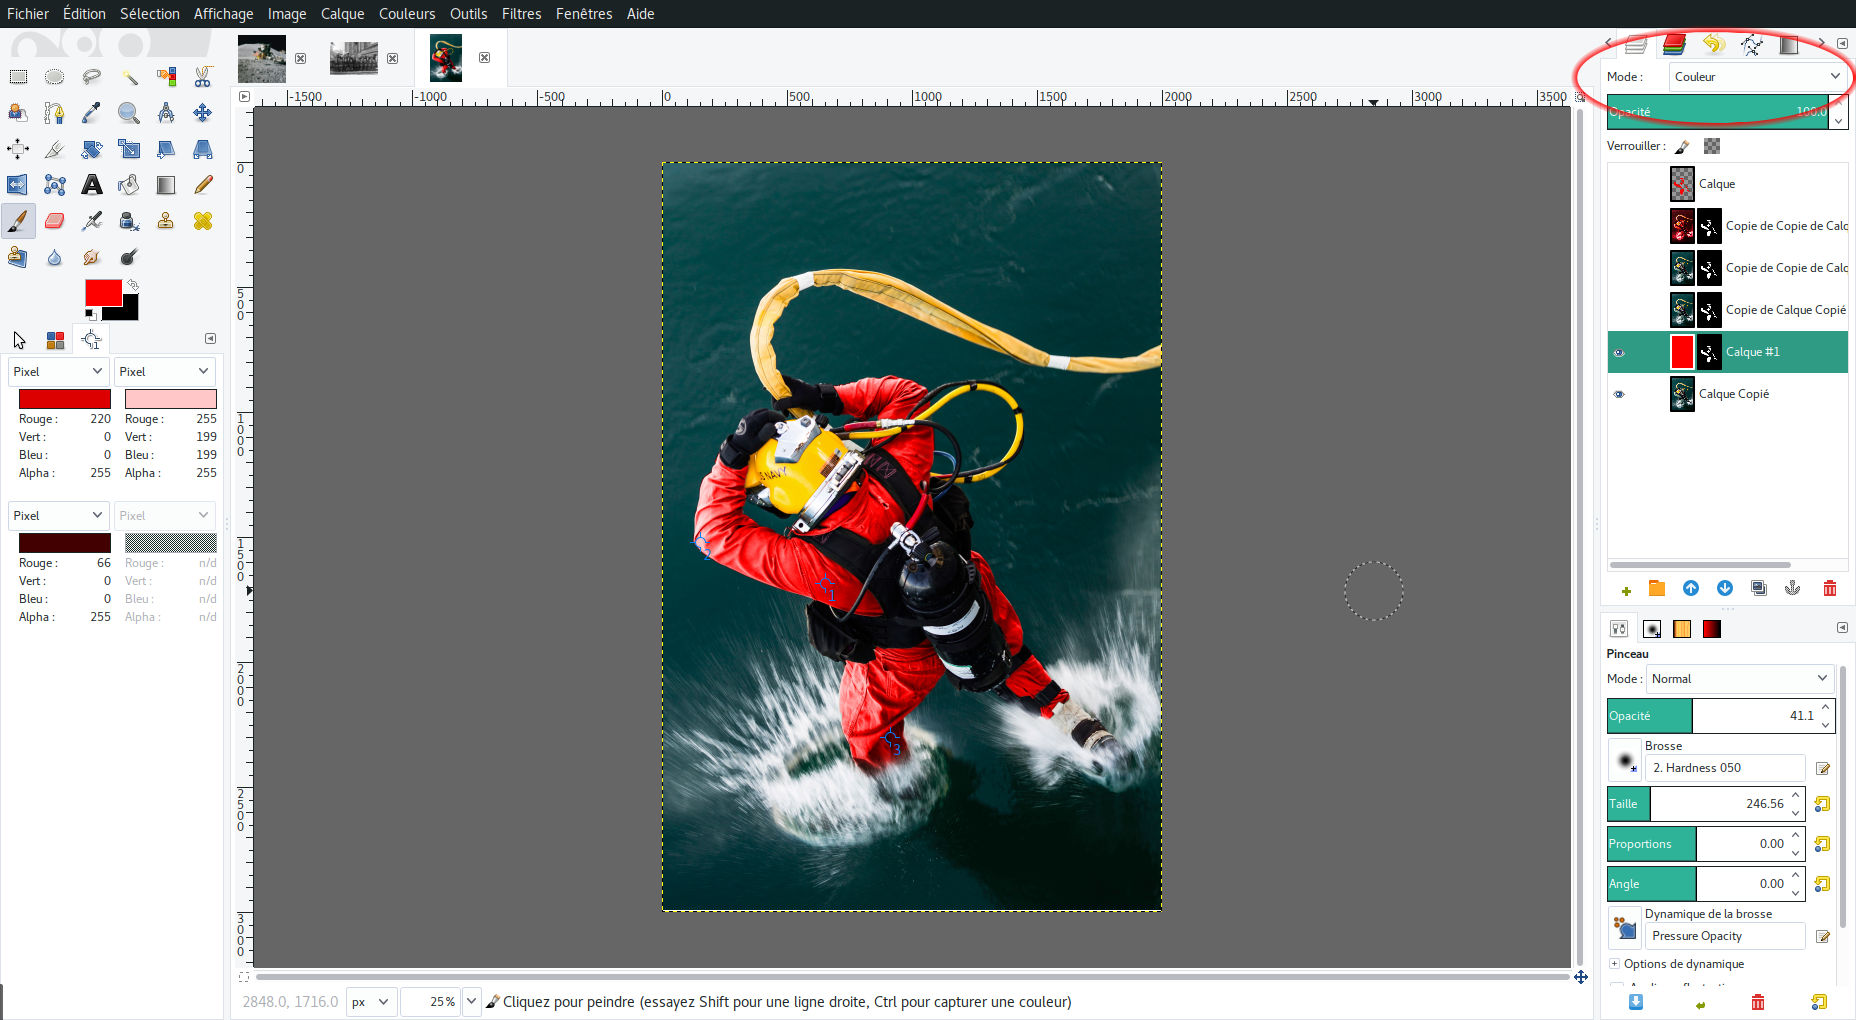
\includegraphics[height=150px]{Images/colours/col8}
			\end{figure}
			}
		\end{enumerate}


	\end{frame}

	\begin{frame}{Gestion des Couleurs}
	\framesubtitle{Par la variation de la balance des blancs}
		Il "suffit" d'adapter les sliders pour les tons sombres, clairs et demi-teintes de l'image jusqu'à avoir la couleur voulue pour chacun.
		\begin{figure}[H]
			\centering
				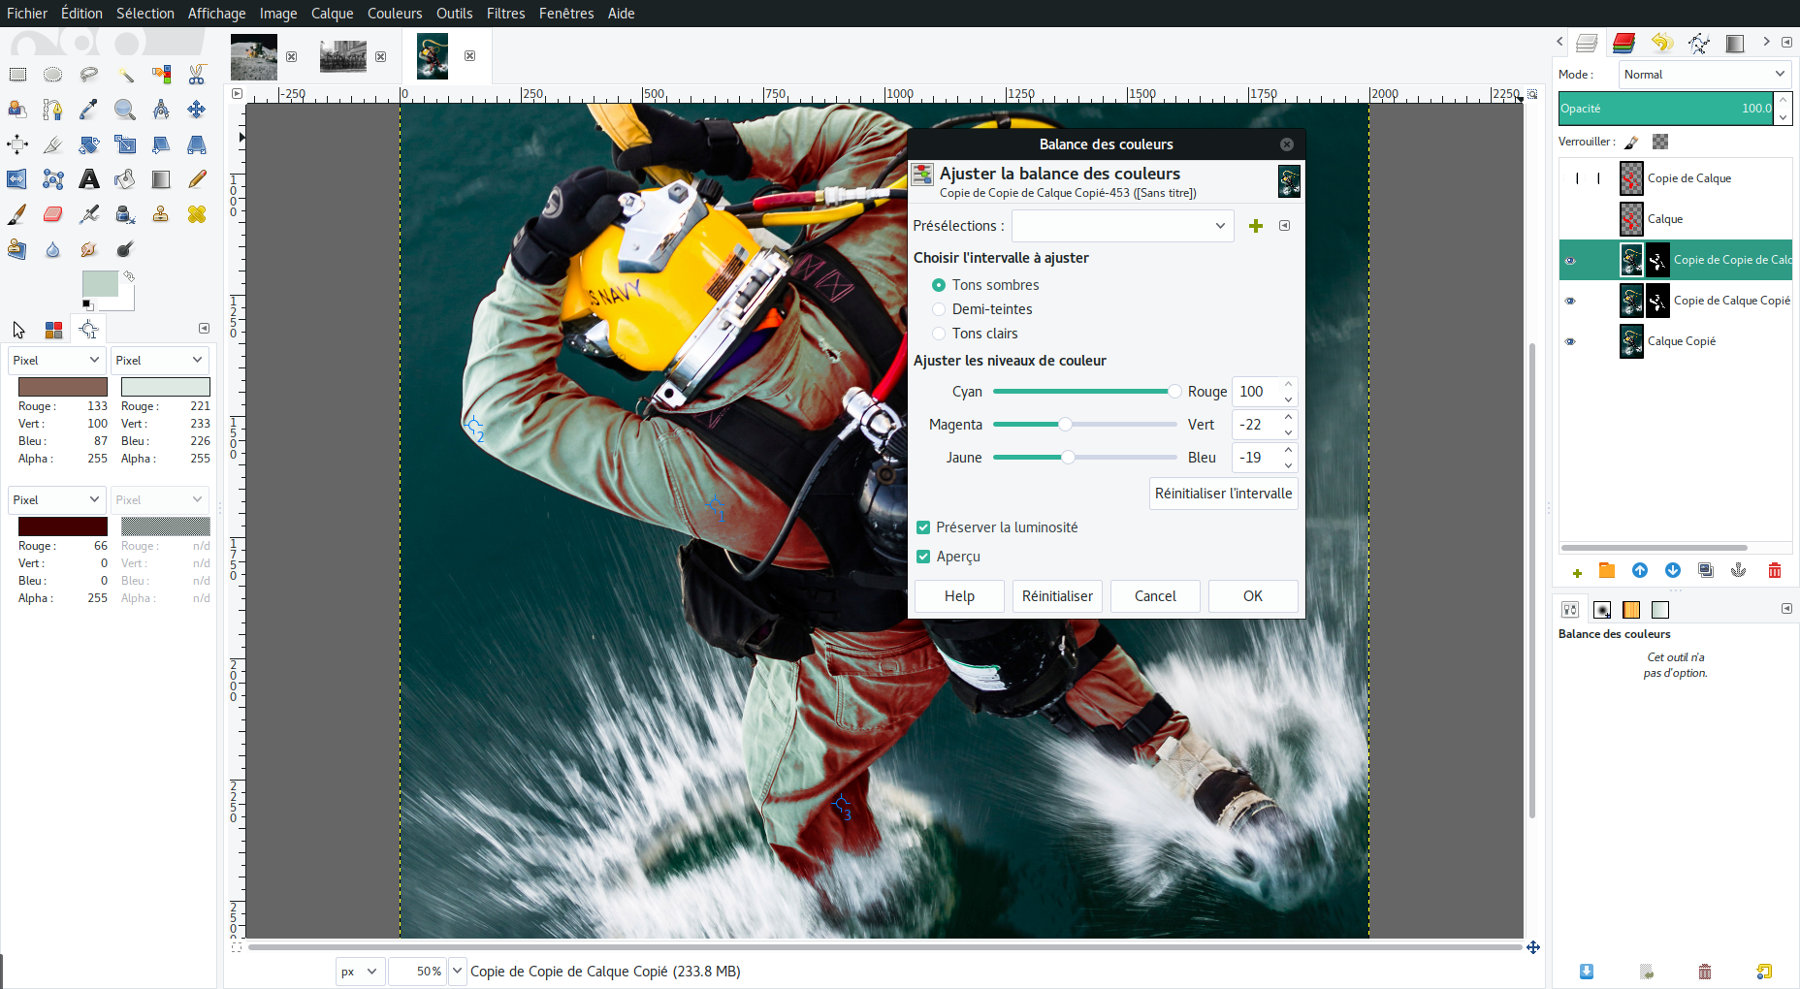
\includegraphics[height=150px]{Images/colours/col9}
			\end{figure}
	\end{frame}

	\begin{frame}{Exercice IV}
		À vous de jouer ! Changez la couleur de la combinaison comme dans l'exemple.
		\begin{itemize}
			\item \href{http://louvainlinux.github.io/atelier-gimp/src/Images/colours/col5.jpg}{Lien de l'image}
		\end{itemize}
	\end{frame}
